\subsection{Vissim}
Vissim provides a microscopic simulation of traffic in a network. In this context microscopic entails that each vehicle is individually modelled and, in a sense, Vissim takes the view of the users of the network.

\subsubsection{Traffic Input}
Vissim is capable of dynamic traffic assignment (DTA) as well as static input. DTA is a method by \cite{Wardrop} in which the traffic flow adapts to the capacity of the network due to a \textit{stochastic user equilibrium} (SUE). 

Vissim can perform this form of traffic input given zones, which are confined and non-overlapping areas of the network, and a matrix describing the relative traffic from each zone to each other zone.

In this project DTA was abandoned on recommendation from DTU Transport professor Otto Anker Nielsen due to the dynamic nature of the traffic signals since, in his experience, odd phenomenon may occur such as unpredictable gridlocks, when adjacent links are fully saturated.

Instead static input was chosen. In static input traffic enters on specific links and traverse the network until an exit link has been reached. Static input is used in combination with routing decisions, which are usually placed on the input links such that each vehicle entering will immediately be assigned a route through the network. For a description of link input sizes and routes used in the simulations, please refer to section \ref{modelling}.

\subsection{Network Elements}

Vissim is highly flexible with regards to network layout description and intersection turning movements can be fine-tuned almost to perfection, given enough time. The network design process is done using a GUI interface where links are joined using connectors.

Links are directed sections of road with $n>=1$ lanes. All lanes have the same direction as the link - the opposite direction is modelled using a parallel link.

Connectors are mostly relevant in intersections where they connect exactly two links, however the lanes connected within the links can be chosen freely.

Vissim maintains a \textit{.inp} file, which contains the most relevant informations necessary to run a simulation including information on links, connectors and routes. 

\subsubsection{Links inputs}
Due to the number of input links and the need to run simulations with various inputs it was decided to implement routines to automate link input definitions.

Since Vissim relies on a text format it is possible to generate strings, which can be inserted in the appropriate section of the \textit{.inp} file.

The format of a link input is:
\begin{verbatim}
INPUT <input_number>
      NAME "<input_description>" LABEL  0.00 0.00
      LINK <link_number> Q <link_contrib> COMPOSITION <comp>
      TIME FROM <t_begin> UNTIL <t_end>
\end{verbatim}

(Vehicles always arrive at the beginning of the link.)

Where the most important fields are the \textit{link\_number}, defining on which link the input occurs, the \textit{link\_contrib}, which is the input quantity in vehicles per hour and finally \textit{t\_begin} and \textit{t\_end} ie. the time period in which this traffic quantity must be generated.

The \textit{comp} variable defines the traffic composition used eg. cars, trucks, buses or a combination. It is possible, but not recommended, to defined multiple inputs on the same link for the same period of time. Since the traffic composition will remain fairly static it is more intuitive to define a single link input for a traffic composition, which defines relative proportions of each possible vehicle type.

\subsubsection{Routing decisions}
\label{routingdecisions}
As mentioned routing decisions are made for vehicles immediately after they enter the system. This is done by placing a route decision point somewhere on an input link and designate a number of exit links, which can be internal links also, so as to generate a set of routes, which can be chosen among from some distribution.

For arterial simulation a general assumption is that most traffic is throughgoing. However, it is unrealistic to omit routes, which are not straight through. As will be seen in the data analysis section (\ref{data}), there are special circumstances to be handled for the two areas being modelled and thus is necessary to provide detailed route choices.

There exist many routes even for small networks when routes are symmetric (albeit using different links). Routes can be designed using the GUI tool provided with Vissim, however since the number of routes that can be taken will grow exponentially in the number of exit links, it is unfeasible to use this approach - especially if different route choice distributions are to be tested. Therefore it was decided to design route generation in the Vissim format, in addition to the before mentioned link input generator.

A routing decisions and the corresponding choice set takes the format:

\begin{verbatim}
ROUTING_DECISION <number> NAME "<description>" LABEL  0.00 0.00
     LINK <origin_link> AT 50.000
     TIME FROM 0.0 UNTIL 99999.0
     NODE 0
      VEHICLE_CLASSES <composition>
     ROUTE     1  DESTINATION LINK <dest_link1>  AT   5.000
     FRACTION <fraction1>
     OVER <connector> <link> ... <connector>
     ROUTE     2  DESTINATION LINK <dest_link2>  AT   5.000
     FRACTION <fraction2>
     OVER <connector> <link> ... <connector>
\end{verbatim}

The \textit{origin\_link} denotes the position of the decision point. The line \textit{VEHICLE\_CLASS...} impose a limit of the vehicles, which are required to select on of the routes of this routing decision. A composition may be a single vehicle type (eg. Car) or a combination (eg. Car, Truck). Next comes a number of lines with route alternatives. The \textit{OVER...} lines describe the path taken from \textit{origin\_link} to \textit{dest\_link}. The first connector must be downstream of - and connected to - the decision point link. Likewise the final connector must be upstream and connected to the destination and the same applies to internal links.

The fractions define the relative distribution of vehicles of the given class or classes, which should take each route. Route fractions can be measured by monitoring license plates at input and exit links, however this is not allowed in Denmark and thus they must be calculated from traffic counts ie. measured turning probabilities in the intersections of the network. DRD supplied traffic counts for this project and the conversion into route fraction is further discussed in section \ref{routefractions}.

In order to enumerate all relevant routes it is necessary to parse the \textit{.inp} file and generate an internal representation of the network as a graph. A route discovery routine was implemented:

\begin{verbatim}
 1: def discover link, path=[[link,nil]], &callback
 2:   for adj_link,conn in link.adjacent
 3:     # avoid loops by checking if the path contain this link
 4:     next if path.map{|l,c|l}.include?(adj_link) 
 5:     
 6:     # assume there exist a valid route using this connector to 
 7:     # reach adj_link; if this is not true, nothing is returned anyhow.
 8:     if adj_link.exit?
 9:       # found an exit link for this path
10:       yield Route.new(path + [[adj_link,conn]]) 
11:    else
12:       # look further
13:       discover(adj_link,path + [[adj_link,conn]],&callback)
14:     end
15:   end
16: end
\end{verbatim}

The discovery routine uses recursion to explore the network and find exit links, which are connected to \verb|link| by a path of links and connectors.

In the initial call only the starting link is given along with a callback, which is invoked by each call of \verb|yield|. 

(The \verb|discover| routine is a so-called generator of Ruby and the first invocation might look like this: \verb+discover(start_link){|route| routes.add(route)}+ where the block is enclosed by \{\} and all routes found from \verb|start_link| are simply stored for later in an array.)

A Vissim route is a sequence of connectors and links and must start and end with the first connector, which is outgoing from the start link, and the connector, which is incoming to the exit link, resp.

In the discovery routine, for each step of the path, a pair is stored which denote the link and by which connector it was reached. This connector thus connects the current link with previous link and therefore the initial path has only one pair where the connector is not defined (nil).

In line 4 a check is made if the adjacent link, which is currently being explored, has already been visited in which case it should be skipped to avoid a loop. In line 8 it is checked wether the adjacent link leads out of the network. If it does we have found a route from the start link otherwise we descend into the recursion and explore the adjacent links of this link.

The \verb|Route.new| invocation, which is performed when an exit link is found, instantiates a new Route object, which enables additional options such as printing the mentioned sequence of connectors links for Vissim, which is more cumbersome with just the raw path.

\subsection{Right-of-Way}
The purpose of traffic signal is to fairly distribute the right-of-way for conflicting traffic motions.  In spite of this traffic signals cannot overcome all situations and rely on road users to enforce themselves some right-of-way rules. This especially becomes relevant when the capacity of the intersection is reached and vehicles become trapped due to a stage change.

Vissim per default allows "collisions" since overlapping links and connectors must be manually prioritized or marked as a conflict area. The existing network was built using previous versions for Vissim, which only supported priority rules (see Figure \ref{fig:priority_rules}). 

\begin{figure}[!ht]
\begin{center}
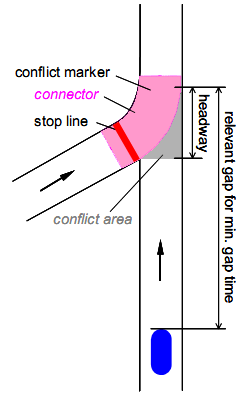
\includegraphics[scale=0.5]{priority_rules.png} 
\end{center}
\caption{From the Vissim manual: illustration of priority rule concepts}
\label{fig:priority_rules}
\end{figure}

In Vissim 5, which was used in this project, there is also the concept of conflict areas, which is recommended over priority rules (the latter remain in Vissim for compatibility) since they are easier to establish and will result in more intelligent driving behaviour. For instance vehicles will avoid entering a conflict area if they can see that it will not be possible to leave it with a certain minimum speed, which will prevent vehicles from clogging up intersections.

Conflict areas and priority rules both rely on threshold values (gap) which road users will use to assess wether it is possible to safely enter a conflict area. The gap is an estimate of the minimum time before the next vehicle from a conflicting link will enter the conflict area.

For the extensions made from Jyllingevej to Roskildevej relevant conflict areas was added for each of the four intersections. The default values in Vissim service pack 6 was used for all conflict areas.

During simulation it became apparent that the priority rules did not prevent collisions in the preexisting intersection so it was decided to replace them with conflict areas. The intersection which had collisions using only priority rules are:

\begin{itemize}
\item Herlev Syghus
\item Hjortespringvej
\item Herlev Hovedgade
\item Mileparken
\item Ejby Industrivej
\item Ejby Industrivej
\item Ejby Torvevej
\item Jyllingevej
\end{itemize}

The intersections with the most observed collisions were Herlev Hovedgade, Hjortespringvej and Herlev Sygehus. It appears that priority rules has difficulties in coping with trapped traffic whereas conflict areas avoid all collisions.
Thus the only priority rules which are carried over from the original model are those for bus stops. 

Conflict areas basically make vehicles in conflicting traffic flows aware of each other so that collisions can be avoided. It is also possible - but no mandatory - to assign a priority. Conflict areas for merging situations should preserve the order of the vehicles and thus have no priority. 

A number of additional situations arise for which the following rules were used:

\begin{enumerate}
\item Left-turning traffic must wait when traffic from the opposite direction - and in the same stage - is going through the intersection
\item When vehicles are trapped in the intersection, waiting for a left turn while the stage changes the vehicles from the next stage, which are in a conflicting motion, must wait for the left-turners to clear even though they have a green light. This is to avoid having traffic stuck in the intersection waiting for their next stage
\item Buses leaving bus stops are always prioritized
\end{enumerate}
